% Copyright 2021 Edoardo Riggio

% Licensed under the Apache License, Version 2.0 (the "License");
% you may not use this file except in compliance with the License.
% You may obtain a copy of the License at

% 	http://www.apache.org/licenses/LICENSE-2.0

% Unless required by applicable law or agreed to in writing, software
% distributed under the License is distributed on an "AS IS" BASIS,
% WITHOUT WARRANTIES OR CONDITIONS OF ANY KIND, either express or implied.
% See the License for the specific language governing permissions and
% limitations under the License.

\documentclass{article}

\usepackage{hyperref, amsmath, graphicx, amssymb}
\usepackage{fancyvrb, newverbs, xcolor, tikz, float}

\usetikzlibrary{positioning}

\graphicspath{{./assets/}}
\definecolor{cverbbg}{gray}{0.93}

\newenvironment{cverbatim}
 {\SaveVerbatim{cverb}}
 {\endSaveVerbatim
  \flushleft\fboxrule=0pt\fboxsep=.5em
  \colorbox{cverbbg}{\BUseVerbatim{cverb}}%
  \endflushleft
}

\newenvironment{lcverbatim}
 {\SaveVerbatim{cverb}}
 {\endSaveVerbatim
  \flushleft\fboxrule=0pt\fboxsep=.5em
  \colorbox{cverbbg}{%
    \makebox[\dimexpr\linewidth-2\fboxsep][l]{\BUseVerbatim{cverb}}%
  }
  \endflushleft
}

\newcommand{\ctexttt}[1]{\colorbox{cverbbg}{\texttt{#1}}}
\newverbcommand{\cverb}
  {\setbox\verbbox\hbox\bgroup}
  {\egroup\colorbox{cverbbg}{\box\verbbox}}
  
\tikzset{%
  every neuron/.style={
    circle,
    draw,
    minimum size=1cm
  },
  neuron missing/.style={
    draw=none, 
    scale=4,
    text height=0.333cm,
    execute at begin node=\color{black}$\vdots$
  },
}

\begin{document}
\begin{titlepage}
    \begin{center}
        \vspace*{1cm}
        
        \Huge
        \textbf{Machine Learning Cheatsheet}
        
        \vspace{0.5cm}
        \LARGE
        
        \vspace{.5cm}
        
        Edoardo Riggio
   		  \vspace{1.5cm}
       
        \vfill
        
        \today
        
        \vspace{.8cm}
          \Large
          Machine Learning - S.P. 2022 \\
        Computer Science\\
        Universit\`{a} della Svizzera Italiana, Lugano\\
        
    \end{center}
\end{titlepage}

\tableofcontents

\newpage

\section{Introduction}
What does it mean "to learn"? We have to different definitions, one from a \textbf{statistical perspective}, and one from a \textbf{computer science perspective}.

\begin{itemize}
	\item \textbf{Statistical Perspective}
	\vspace{.2cm} \\
	Vast amounts of data are being generated in many fields. The statistician's job is to make sense of this data, extract meaningful patterns and trends, and understand "what the data says". This approach is also known as \textbf{learning from data}.
	
	\item \textbf{Computer Science Perspective}
	\vspace{.2cm} \\
	The field of machine learning is concerned with how to construct computer programs that automatically improve with experience.
\end{itemize}

\subsection{Mitchell's Formalisation}
A computer program is said to learn from \textbf{experience $E$} -- concerning some class of \textbf{task $T$}, and \textbf{performance measurement $P$} -- if its performance at task $T$, as measured by $P$, improves with experience $E$.

\subsection{Models}
\subsubsection{White Box Model}
The problem's physical laws and structural parameters are known in this case. A family equation can be derived.

\subsubsection{Grey Box Model}
The physical laws are known in this case, and at least one parameter is unknown. A family of equations can be derived, but the parameters need to be identified.

\subsubsection{Black Box Model}
In this case, the physical laws are unknown. A family of equations cannot be derived.

\subsection{Measures and Measurements}
The operation of measuring an unknown quantity $x_0$ can be modeled as taking an instance -- i.e., a \textbf{measurement} -- $x_i$ at time $i$, with an ad-hoc sensor $S$. \\ \\
Although $S$ has been suitably designed and realized, the physical elements that compose it are far from ideal and introduce uncertainties in the measurement process. As a result, $x_i$ only represents an estimate of $x_0$.

\subsection{Types of Models}
\subsubsection{Additive Model}
The measurement process can be modeled as:
\[ x = x_0 + \eta ~~~~~\text{where}~\eta = f_n(0, \sigma^2_\eta) \]
Where $\eta$ is an independent and identically distributed random variable, the model assumes that the i.i.d. noise does not depend on the working point $x_0$.

\subsection{Multiplicative Model}
The measurement process can be modeled as:
\[ x = x_0 (1 + \eta) ~~~~~\text{where}~\eta = f_n(0, \sigma^2_\eta) \]
Where $\eta$ is an independent and identically distributed random variable, the noise, in this case, depends on the working point $x_0$. In absolute terms, the impact of the noise on the signal is $x_0 \eta$, but the relative contribution is $\eta$ -- which does not depend on $x_0$.

\subsection{Supervised Learning}
In a supervised learning framework, we have the following elements: a \textbf{concept to learn}, a \textbf{teacher}, and a \textbf{student}.

\subsubsection{Regression}
The goal of regression is to determine the function that explains the given instances -- \textbf{measuremets}. The student proposes a family of models $f(\theta, x)$, and after a learning procedure, the "best" model $f(\hat \theta, x)$ is found.

\subsubsection{Classification}
The goal of classification is to determine the function -- \textbf{model} -- that partitions the input -- \textbf{measurements} -- into classes. The student proposes a family of models $f(\theta, x)$, and after a learning procedure, the "best" model $f(\hat \theta, x)$ is found.

\subsubsection{Prediction}
The goal of prediction is to tell us which data -- \textbf{measurements} -- will come next, possibly along with a confidence level. The student proposes a family of models $f(\theta, x)$, and after a learning procedure, the "best" model $f(\hat \theta, x)$ is found.

\subsection{Features}
We might want to extract features from the measurements to ease the learning task. The features must:
\begin{itemize}
	\item Provide a compact representation of inputs
	\item Be particularly advantageous if we have prior information to take advantage of
	\item Be reduced to a minimal set before processing them for task solving
\end{itemize}

\subsection{Unsupervised Learning}
The goal of unsupervised learning is to build a representation of data. During its operational life, given an input, the machine provides information that can be used for decision-making.

\section{Linear Regression}
To prepare a linear regression model, several techniques can be used. The most popular being the \textbf{Least Mean Square (LMS)}, and the \textbf{Gradient Descent}. \\ \\
Linear models are good when we have the following conditions:
\begin{itemize}
	\item The data is generated by a linear model
	\item The dataset is small
	\item The data is sparse
	\item The uncertainty is high
\end{itemize}

\subsection{Muliple Linear Regression}
We are given a set of points:
\[ \{ (x_1, y_1), (x_2, y_2), \dots, (x_n, y_n) \} ~~~~~ \text{where}~x \in \mathbb{R}^d, y \in 	\mathbb{R} \]
This is known as the \textbf{training set}. We now assume that the unknown function that generates the data is linear. Moreover, we assume that there is a gaussian uncertainty affecting the measurements. The model is given as:
\[ y(x) = \theta^0_1 + \theta^0_2 z_2 + \dots + \theta^0_d z_d ~~~~ \text{where}~\theta^0 \in \mathbb{R}, \eta = N(0, \sigma^2_\eta) \]
Which can be written in its canonical form:
\[ y(x) = x^T \theta^0 + \eta ~~~~~ \text{where}~x^T = \begin{bmatrix} 1 & z_2 & \cdots & z_d \end{bmatrix}, \theta^{0^T} = \begin{bmatrix} \theta^0_1 & \theta^0_2 & \cdots & \theta^0_d \end{bmatrix} \]
Both the optimal parameters and the variance of the noise are unknown. Since we know that the system model is linear, the family of models which best fits the data is:
\[ \hat y(x) = f(\theta, x) = x^T \theta \]
In order to determine the best parameters, we estimate them:
\[ f(\hat \theta, x) = x^T \hat \theta \]

\subsubsection{Least Mean Square}
The main idea of this procedure is to select the linear function that minimizes the average distance between the given points and the linear function. \\ \\
The \textbf{performance function} of this method is the following:
\[ V_n(\theta) = \frac{1}{n} \sum^n_{i=1}(y(x_i) - f(\theta, x_i))^2 \]
Therefore, the parameter vector $\hat \theta$ minimizing the performance function is the following:
\[ \hat \theta  = \arg\min_{\theta \in \Theta} V_n(\theta) \]

\subsubsection{Parameter Estimation}
By grouping the data into vectors $X$ -- of all $x$ values -- and $Y$ -- of all $y$ values, we can rewrite the formula above in its canonical form:
\begin{align*}
	V_n^*(\theta) &= \sum^n_{i=1} (y(x_i) - x^T_i \theta)^2 \\
	&= (Y - X\theta)^T (Y - X\theta) 
\end{align*}
\textbf{Stationary points} are those for which:
\[ \frac{\partial V_n^*(\theta)}{\partial \theta} = -2X^T Y + 2X^T X \theta = 0 \]
Therefore, the parameter vector $\hat \theta$ minimizing the performance function is the following:
\[ \hat \theta = (X_TX)^{-1}X^TY \]
And the best approximating model is:
\[ f(\hat \theta x) = x^T\hat\theta \]

\subsection{Performance at Task}
In order to test the model, we need to use another set of unseen data. This is because the \textbf{performance at task}:
\[ V_n(\hat\theta) = \frac{1}{n} \sum^n_{i=1}(y(x_i) - f(\theta, x_i))^2 \]
It is biased to the training set. For this reason, we consider another set of data -- different from the training set -- and call it \textbf{test set}:
\[ \{ (\bar x_1, \bar y_1), (\bar x_2, \bar y_2), \dots, (\bar x_l, \bar y_l) \} \]
And evaluate the performance at task on it:
\[ V_l(\hat\theta) = \frac{1}{l} \sum^l_{i=1}(\bar y_i - \bar x^T\hat\theta)^2 \]

\subsection{Cross-Validation}
Cross-validation provides a means to assess the performance of a model. This method can also be considered for model selection -- with some care. In the latter case, we consider the model that minimizes
\[ V_l(\hat\theta) = \frac{1}{l} \sum^l_{i=1}(\bar y_i - \bar x^T\hat\theta)^2 \]

\subsection{Properties}
Under the linear framework presented earlier, it can be proved that both implications hold true:
\[ \lim_{n \rightarrow \infty} \hat\theta = \theta^0 \]
\[ \lim_{l \rightarrow \infty} V_l(\hat\theta) = \sigma^2_\eta \]
In addition, assuming that $n$ training couples are given, then it can be proved that:
\[ Var(\hat\theta) = (X^TX)^{-1}\sigma^2_\eta ~~~~~ \text{with}~\hat\sigma^2_\eta = \frac{1}{n - d} \sum^n_{i = 1}(y(x_i) - f(\hat\theta, x_i))^2 \]
If a parameter is smaller than twice its standard deviation, it must be set to 0. After which, we re-evaluate the performance and decide whether to keep it. This is known as \textbf{Occam's razor strategy}.

\subsection{Ridge Regression}
Ridge regression aims at pushing as many parameters as possible towards zero. This is done by adding a shrinking penalty to the loss function. The \textbf{MSE} training performance mesure
\[ V_n(\theta) = \frac{1}{n} \sum^n_{i=1}(y_i - x_i^T\theta)^2 \]
Now becomes
\[ V_{Ridge}(\theta) = \frac{1}{n} \sum^n_{i=1}(y_i - x_i^T\theta)^2 + \lambda \sum^d_{i=2}\theta^2_i \]
Where $\lambda$ is a hyperparameter weighting the two contributions. A smaller $\lambda$ gives more importance to accuracy, while a high $\lambda$ priviledges a smaller number of parameters in the model. A tradeoff can be obtained by estimating and appropriate $\lambda$ thanks to the \textbf{validation set}.

\subsection{Lasso Regression}
Lasso regression also aims at pushing as many parameters as possible towards zero. In this case, however, we penalize the parameter itself rather than its square. The \textbf{MSE} now is:
\[ V_{Lasso}(\theta) = \frac{1}{n} \sum^n_{i=1}(y_i - x_i^T\theta)^2 + \lambda \sum^d_{i=2}|\theta_i| \]
The optimization problem is not convex anymore, and the loss function is not differentiable. This makes the problem computationally complex and solvable only via optimization techniques such as quadratic programming.
 
\subsection{Final Prediction Error}
The expected prediction error is computed as follows:
\[ FPE = \frac{n+d}{n-d}\sum^n_{i=1}(y(x_i) - f(\hat\theta, x_i))^2 \]
This measurement can be used for both model selection -- only on hierarchical family of models, and for assessing the performance of unseen data.
 
\section{Non-Linear Regression}
To determine the stationary points of a differentiable function we use the following minimization problem:
\[ \hat\theta = \arg \min_{\theta \in \Theta} V_n(\theta) \]
This minimization is carried out by a \textbf{gradient descent-based procedure}.
 
\subsection{Gradient-Based Optimization}
Given a generic convex and differentiable scalar function $y = f(x)$, we do the following to determine the unique stationary point. \\ \\
We start from an initial point $x(0) = x_0$ and start moving along the gradient in the direction minimizing the loss function. To do so we use the following formula:
\[ \theta_{i+1} = \theta_i - \varepsilon_L \frac{\partial V_n(\theta)}{\partial \theta}|_{\theta_i} \]
The minimization procedure applied to a non-linear function -- and based on a training set -- is also known as \textbf{learning procedure}. \\ \\
When minimizing, we might encounter what is known as the \textbf{identifiability problem}. This happens when the function to be optimized is not convex, and there are several local or global minima in the function.

\subsection{Structural Risk}
The structural risk of the estimated model is its generalization ability. To compute the function's generalization ability, we use the following formula:
\[ \bar V(\hat\theta) = \int L(y, f(\hat\theta, x)) p_{x, y} dxy \]
Where $L$ is the \textbf{loss function}. The risk associated with the model's generalization ability can be decomposed into three terms:
\[ \bar V(\hat\theta) = (\bar V(\hat\theta) - \bar V(\theta^0)) + (\bar V(\theta^0) - V_I) + V_I \]

\subsubsection{Inherent Risk}
The inherent risk depends entirely on the structure of the learning problem. This term can be improved only by improving the problem, such as reducing the noise caused by the measurement instruments. \\ \\
The inherent risk is computed as:
\[ V_I \]

\subsubsection{Approximation Risk}
The approximation risk depends on how close the approximating family of models is to the function generating the data ($g(x)$). We can use a more appropriate family of models to reduce this risk. \\ \\
The approximation risk is computed as:
\[ \bar V(\theta^0) - V_I \]

\subsubsection{Estimation Risk}
The estimation risk depends on the effectiveness of the learning procedure. We can use a more effective learning procedure to reduce this risk. \\ \\
The estimation risk is computed as:
\[ \bar V(\hat\theta) - \bar V(\theta^0) \]

\section{Feedforward Neural Networks}
A neural network has the following structure \\ \\

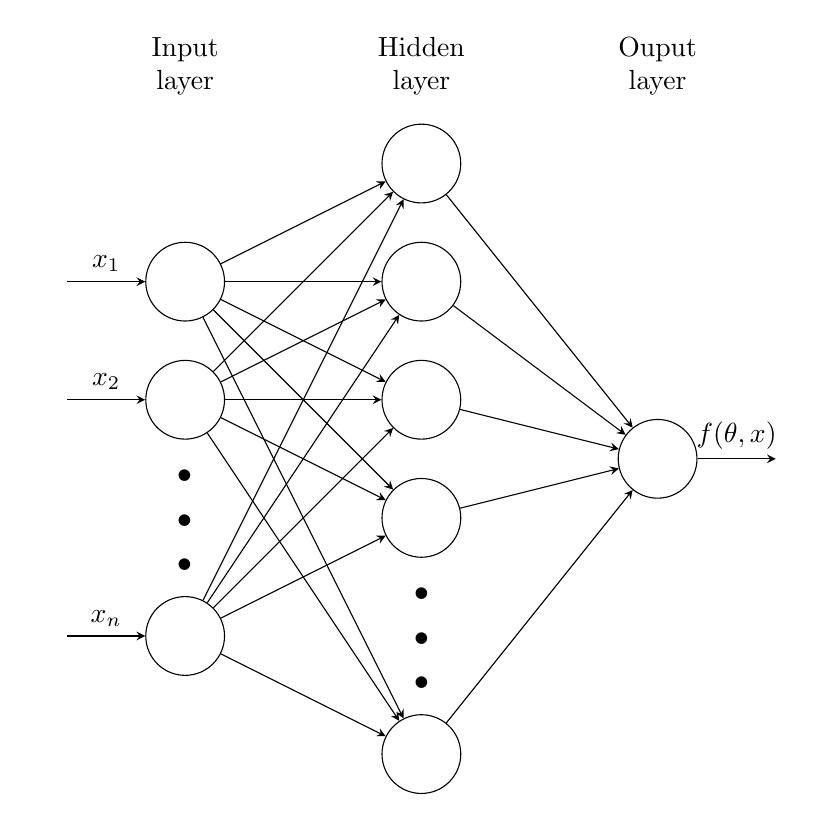
\begin{tikzpicture}[x=1.5cm, y=1.5cm, >=stealth]
\foreach \m/\l [count=\y] in {1,2,missing,3}
  \node [every neuron/.try, neuron \m/.try] (input-\m) at (0,1.5-\y) {};

\foreach \m [count=\y] in {1,2,3,4,missing,5}
  \node [every neuron/.try, neuron \m/.try ] (hidden-\m) at (2,2.5-\y) {};

\node [every neuron/.try, neuron 1/.try ] (output-1) at (4,1-2) {};
\foreach \l [count=\i] in {1,2,n}
  \draw [<-] (input-\i) -- ++(-1,0)
    node [above, midway] {$x_\l$};

\draw [->] (output-1) -- ++(1,0)
  node [above, midway] {$f(\theta, x)$};

\foreach \i in {1,...,3}
  \foreach \j in {1,...,5}
    \draw [->] (input-\i) -- (hidden-\j);

\foreach \i in {1,...,5}
  \draw [->] (hidden-\i) -- (output-1);

\foreach \l [count=\x from 0] in {Input, Hidden, Ouput}
  \node [align=center, above] at (\x*2,2) {\l \\ layer};
\end{tikzpicture} \\ \\
Each connection between neurons has a weight of $w_n$. Moreover, the overall weight of a sigle neuron is computed as:
\[ a_t = \sum^n_{i=1}x^i w^i \]
Each neuron in the hidden layer has an activation function. This activation function can be of several different types:

\begin{itemize}
	\item \textbf{Sigmoidal}
	\vspace{.2cm} \\
	This activation function is mainly used by the neurons of the hidden layer. The sigmoidal formula is:
	\[ Sig(x) = \frac{1}{1 + e*{-x}} \]
	
	\item \textbf{Hyperbolic Tangent}
	\vspace{.2cm} \\
	This activation function is an alternative to the sigmoidal activation function. This function is useful when we have back-propagation. The hyperbolic tangent formula is:
	\[ HT(x) = \frac{e^x-e^{-x}}{e^x+e^{-x}} \]
	
	\item \textbf{Linear}
	\vspace{.2cm} \\
	The neurons of the output layer mainly use this activation function.
\end{itemize}

\subsection{Universal Approximation Theorem}
A feedforward neural network with a single hidden layer containing a finite number of neurons and a linear output neuron approximates any continuous function defined on compact subsets.

\subsection{Early Stopping}
The idea of early stopping is to start from an over-dimensioned network and try to find where the models start diverging.

\begin{center}
	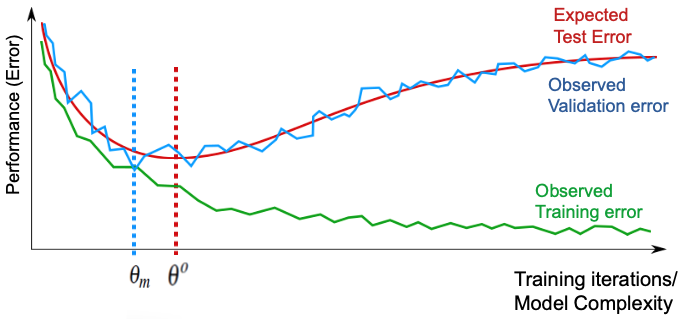
\includegraphics[width=10cm]{early_stopping.png}
\end{center}
To evaluate the model, we use another set of data called \textbf{validation set}. We cannot use the test set for the model selection during training. Otherwise, the model performance assessment would be biased.

\subsection{Splitting the Data}
We apply a ratio (application-dependent) to split the data we have -- which has length $n$, we apply a ratio (application-dependent). This ratio is computed in the function of:

\begin{itemize}
	\item The size of $n$
	\item The complexity of the model
\end{itemize}
For example:
\[ n = 1,000 \rightarrow Tr = 70\%,~ V = 15\%,~ Te = 15\% \]
\[ n = 1,000,000 \rightarrow Tr = 99\%,~ V = 0.5\%,~ Te = 0.5\% \]

\section{Classification Problem}
Given an input vector $x$, and a set of classes $C_1, C_2, \dots, C_k$, we wish to assign $x$ to the most appropriate class. In classification, $y$ assumes a categorical value.

\subsection{Binary Classifier}
Given an input vector $x$ of two features and two classes, we divide the features in a binary manner -- i.e., either it is in one group or the other.

\begin{center}
	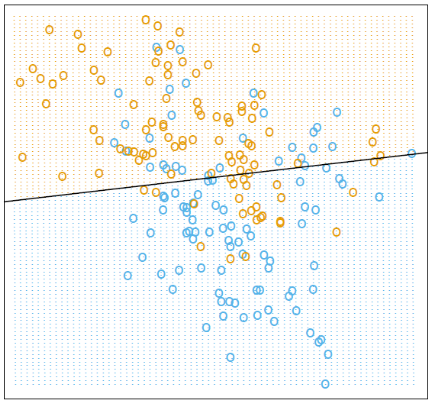
\includegraphics[width=6cm]{binary_classification.png}
\end{center}
Given a training set, we obtain the following estimated parameter:
\[ \hat\theta = (X^TX)^{-1}X^TX \]
And given a new $x$, we evaluate the following discriminant function:
\[ f(\hat\theta, x) = x^T\hat\theta \]
If the discriminant value is above $0.5$, then $x$ will be part of one group. Otherwise, $x$ will be part of the other group.

\subsection{Bayes Classifier}
The Bayes classifier deals with multi-class problems. Here we assign a probability to each class and select the one that maximizes such probability.
\[ Pr(Y = k|X = x) \]
Where $X$ and $Y$ are two random variables. The Bayes theorem described above provides us with a way to express the posterior conditional probability as:
\[ Pr(Y = k|X = x) = \frac{Pr(X = x|Y = k) \cdot Pr(Y = k)}{Pr(X = x)} \]
Where $Pr(Y = k|X = x)$ is the \textbf{posterior probability}, $Pr(X = x|Y = k)$ is the \textbf{likelihood}, $Pr(Y = k)$ is the \textbf{prior probability}, and $Pr(X = x)$ is the evidence.

\begin{center}
	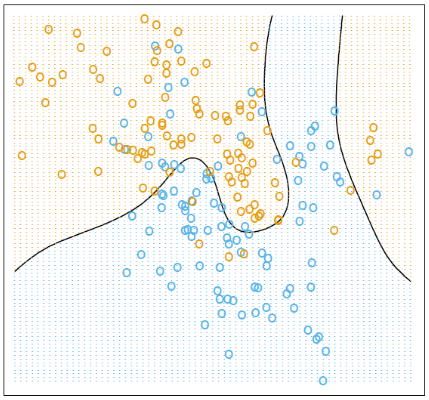
\includegraphics[width=6cm]{bayes_classification.png}
\end{center}
This classifier is said to be na\"ive. It is because it makes the strong assumption of independence among the features. The Bayes classifier is optimal if the premises and known probabilities are met.

\subsection{K-Nearest Neighbour Classifier}
This classifier looks at the $k$-nearest neighbors of point $x$ to make the classification decision. For example, the Euclidean distance can be used to determine the class.

\begin{center}
	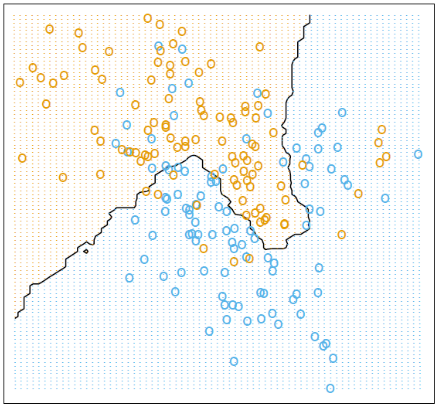
\includegraphics[width=6cm]{nearest_neighbors.png}
\end{center}
No training phase is required in this case, but we have a high computational cost in evaluating the distances.

\subsection{Linear Discriminant Analysis}
Linear Discriminant Analysis (LDA) is a robust way to solve the classification problem and find a separating boundary. \\ \\
Here we reformulate the Bayes theorem in terms of probability density functions. Thus:
\[ Pr(Y = k|X = x) = \frac{\pi_kf_k(x)}{\sum^K_{l=1} \pi_lf_l(x)} \]
Where $\pi_k = Pr(Y=k)$ is the \textbf{prior probability}, and $f_k(x)$ represents the \textbf{likelihood of the $k$-th class} and is defined as:
\[ f_k(x) = Pr(X=x|Y=k) \]

\subsubsection{One-Dimensional Setting}
If we consider a one-dimensional setting and Gaussian distributed classes:
\[ f_k(x) = \frac{1}{\sqrt{2\pi} \cdot \sigma_k}e^{-\frac{1}{2}\left( \frac{x-\mu_k}{\sigma_k} \right)^2} \]
Which can be represented graphically as:

\begin{center}
	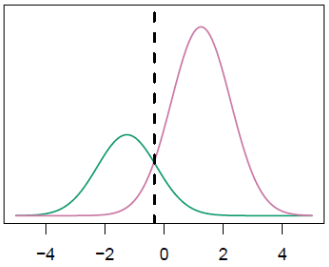
\includegraphics[width=4cm]{lda.png}
\end{center}
In the case of a scalar $x$ and identical variances, the Bayes formula becomes:
\[ Pr(Y = k|X = x) = \frac{\pi_k\frac{1}{\sqrt{2\pi} \cdot \sigma}e^{-\frac{1}{2}\left( \frac{x-\mu_k}{\sigma} \right)^2}}{\sum^K_{l=1} \pi_l\frac{1}{\sqrt{2\pi} \cdot \sigma}e^{-\frac{1}{2}\left( \frac{x-\mu_l}{\sigma} \right)^2}} \]
To obtain the line that separates the classes, we are looking for the maximum of the above probability. We simplify the formula by taking the log and removing the constant terms. The discriminant function now becomes:
\[ \delta_k(x) = x \cdot \frac{\mu_k}{\sigma^2} - \frac{\mu^2_k}{2\sigma^2} + \log(\pi_k) \]
The decision boundary between two classes satisfies the equation $\delta_k(x) = \delta_i(x)$.

\subsubsection{Vector Space Setting}
In the case of vectors, we will have the following formula:
\[ f(x) = \frac{1}{(2\pi)^{p/2}|\sum|^{1/2}} e^{-\frac{1}{2}(x-\mu)^T \sum^{-1}(x-\mu)} \]
Which can be represented graphically as:

\begin{center}
	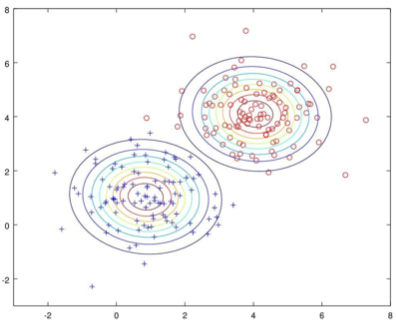
\includegraphics[width=4cm]{lda_vectors.png}
\end{center}
Now the linea discriminant will become:
\[ \delta_k(x) = x^T \Sigma^{-1} \mu_k - \frac{1}{2}\mu^T_k \Sigma^{-1}\mu_k + \log \pi_k \]
With two classes, the LDA coincides with the linear regression classification method. Here, the decision boundary between two classes satisfies the equation $\delta_k(x) = \delta_i(x)$.

\subsection{Perceptron}
The perceptron algorithm was invented to solve pattern classification problems. This method works well on linearly separable classes, and its parameters can be learned. \\ \\
The architecture of a perceptron is that of a neural network with a single neuron with a \textit{Heaviside} activation function. After a random assignment of weights, these are iteratively updated during the training procedure.
\[ w^j_{t+1} = w^j_t - \varepsilon_L(y_i - f(w_t, x_i))x^j_i \]
The algorithm will converge to the optimal parameter -- if the problem is linearly separable.

\subsection{Classification with Feedforward Neural Networks}
Given a performance function:
\[ V_n(\theta) = \frac{1}{n} \sum^n_{i = 1} L(y_i, f(\theta, x_i) \]
We determine the parameter estimate by solving the following minimization problem:
\[ \hat\theta = \arg\min_{\theta \in \Theta} V_n(\theta) \]
This is carried out by the following learning procedure:
\[ \theta_{i+1} = \theta_i - \varepsilon_L \frac{\partial V_n(\theta)}{\partial\theta} \Big|_{\theta = \theta_i} \]
And finally, obtain the classifier:
\[ f(\hat\theta, x) \]

\subsection{Logistic Regression}
Linear classifiers derived as extensions of the regression methods neither provide a bounded output nor a probabilistic interpretation. \\ \\
Logistic regression aims at training the network's parameters so that a probabilistic network supports the sigmoidal output.

\section{Model Performance}
\subsection{Quality Assessment if the Solution}
There are several different ways to estimate the performance of a classifier.

\subsubsection{Apparent Error Rate}
This method computes the empirical risk to estimate the structural one. The set $Z_n$ is used to infer the model and estimate its accuracy performance. \\ \\
AER is a strongly optimistically biased estimate unless $n$ is very large.

\subsubsection{Crossvalidation}
Crossvalidation estimates the generalization error $\bar V(\hat\theta)$ on a new dataset. The sets $S_D$ and $S_E$ are generated by \textbf{randomly} splitting $Z_n$ into two disjoint subsets. we use $S_D$ as the \textbf{training set}, and $S_E$ as the \textbf{test set}. \\ \\
This method can be considered an unbiased estimate if $S_E$ is large enough.

\subsubsection{K-Fold Crossvalidation}
This method randomly splits $Z_n$ into $k$ disjoint subsets of equal size. For each subset, the other $k-1$ remaining subsets are merged to form $S_D$, and the $k$ subset is used as $S_E$. The resulting $k$ estimates are averaged.

\subsubsection{Leave-One-Out}
In this method, $S_E$ contains one pattern of $Z_n$, and $S_D$ contains the remaining $n - 1$ patterns of $Z_n$. The procedure iterates $n$ times, holding out each pattern in $Z_n$. The resulting $n$ estimates are averaged. \\ \\
This is a simplification of K-CV. The estimates from each fold are highly correlated. Thus, the estimate has a significant variance.

\subsubsection{Bootstrap Method}
If we have a very small dataset, we use this method. The algorithm is similar to Leave-One-Out. Although, in this case, patterns are selected from $Z_n$ \textbf{with replacement}. \\ \\
This method underestimates the test error $\bar V(\hat\theta)$

\subsection{Model Validity}
Model validity is used to define which model is the best one.

\subsection{Test on Residuals}
The verification of the hypothesis $E[\varepsilon] = 0$ requires a test on the sample mean. The null hypothesis we consider is $H_0 : E[\varepsilon] = 0$, while the alternate hypothesis is $H_1 : E[\varepsilon] \not = 0$. To see which hypothesis holds, we need to design a statistic. \\ \\
Under the \textbf{null hypothesis} $H_0$, the Central Limit Theorem grants the T-Student statistic to follow a normal distribution. We compute $T$ as such:
\[ T = \frac{\bar \varepsilon}{\sqrt{\frac{s^2}{l}}} \sim N(0,1) \]
\[ \bar\varepsilon = \frac{1}{l} \sum^l_{i = 1} \varepsilon_i \]
\[ s^2 = \frac{1}{l} \sum^l_{i = 1} \varepsilon^2_i \]
If $T$ is outside of the 95\% confidence interval -- i.e., [-1.96, 1.96] -- then we reject the null hypothesis $H_0$. \\ \\
Something similar can be done to check if one model is statistically better than the other. In this case we consider the null hypothesis to be:
\[ H_0 : Var[\varepsilon_a] = Var[\varepsilon_b] \]
\[ H_1 : Var[\varepsilon_a] \not = Var[\varepsilon_b] \]
We reject the null hypothesis if $T$ -- or rather a slightly modified version -- is out of the 95\% confidence interval. This means that the two models are different. Now that we know they are different, we compute their variances to determine which model is the best. The model with the lowest variance is the best one.

\subsection{Assessing Anomaly detection Methods}
An anomaly detector is a classifier that processes data streams looking for anomalies.

\subsubsection{Confusion Matrix}
A confusion matrix describes the nature of the classification performance.

\begin{center}
	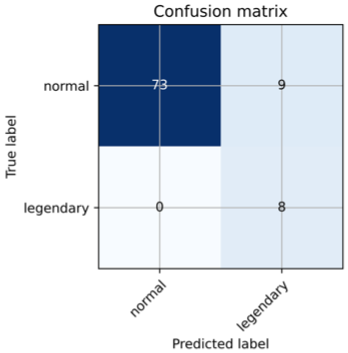
\includegraphics[width=4cm]{assets/confusion_matrix.png}
\end{center}
Where \textit{normal-normal} are the \textbf{true positives}, \textit{normal-legendary} are the \textbf{false negatives}, \textit{legenday-normal} are the \textbf{false positives}, and \textit{lagendary-legendary} are the \textbf{true negatives}. \\ \\
Given this truth table, we can compute some probabilities:

\begin{itemize}
	\item \textbf{True Positive Rate}
	\[ TPR = \frac{\#\{ \text{true positives} \}}{\#\{ \text{legendary samples} \}} \]
	
	\item \textbf{False Positive Rate}
	\[ FPR = \frac{\#\{ \text{false positives} \}}{\#\{ \text{normal samples} \}} \]
	
	\item \textbf{False Negative Rate -- Miss Rate}
	\[ FNR = 1 - TPR \]
	
	\item \textbf{True Negative Rate -- Specificity}
	\[ TNR = 1 - FPR \]
	
	\item \textbf{Precision}
	\[ P = \frac{\#\{ \text{true negatives} \}}{\#\{ \text{detections} \}} \]
	
	\item \textbf{Recall}
	\[ R = TPR \]
\end{itemize}
To correctly assess the method performance, it is necessary to consider at least two indicators:

\begin{itemize}
	\item \textbf{Accuracy}
	\[ A = \frac{\#\{ \text{true negatives}\} + \#\{\text{false negatives} \}}{\#\{ \text{samples} \}} \]
	
	\item \textbf{F1 Score}
	\[ \frac{2 \cdot \#\{ \text{true negatives}\}}{\#\{ \text{detections} \} + \#\{ anomalies \}} \]
\end{itemize}
The values for the accuracy and the F1 score are 1 when we have an ideal detecting method.

\section{Deep Learning}
Deep learning flourished thanks to significant advances in computational power and the cost-effective availability of big data for training. \\ \\
Deep learning can have several applications:

\begin{itemize}
	\item Detect/classify different elements within a scene
	\item Generate new images that look extremely realistic
	\item Make decisions with the same skills and creativity as humans
\end{itemize}
\subsection{Representation Learning}
In more traditional approaches, hand-crafted features and then fed to the neural network. Instead, in the case of deep learning, the features are directly learned by the neural network. \\ \\
In representation learning, there is a hierarchical abstraction of the features. These features are low- mid-, and high-level. After the extraction, these features are fed to the classifier.

\subsection{Convolutional Neural Networks}
CNNs take advantage of the space affinities existing among neighbors. These networks are made up of many different layers. Each layer computes a higher abstract representation of the image while at the same time making the image shrink at each step -- done by \textbf{convolutional} and \textbf{pooling} layers. \\ \\
The feature maps are concatenated in a single vector and fed to a feed-forward neural network.

\subsubsection{Convolutional Layer}
Convolutional layers evaluate the affinities of pixels based on the principle of locality. A \textbf{receptive field} is applied to the image with a certain \textbf{stride}. This results in an output image:
\[ M = I \cdot K \]
Where $I$ is the \textbf{original matrix}, and $K$ is the \textbf{filter} that contains the parameters to be learned.

\begin{center}
	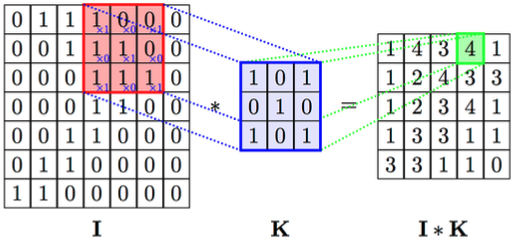
\includegraphics[width=6cm]{assets/convolutional.png}
\end{center}
As each feature is learned, many filters can be applied in parallel and the filter $K$ changes. After the convolution process, each filter $K$ will have provided with a different \textbf{feature map}. Another characteristic of these convolutional layers is that they offer some \textbf{local translation invariance property}. This means that it doesn't matter if the relevant parts of the image move around.

\subsubsection{Pooling Layer}
Pooling layers reduce the image size based on some specific rules. The pooling operators are:

\begin{itemize}
	\item \textbf{Max Pooling}
	Given a square of -- say -- 4 different values, the pixel with the maximum one is carried to the next layer. This means that from 4 pixels, we only retain 1 (which has the maximum value).
	
	\item \textbf{Average Pooling}
	This is done in the same way as the max pooling. Although, in this case, the value carried to the next layer is the average between the pixels values of the current image.
\end{itemize}

\begin{center}
	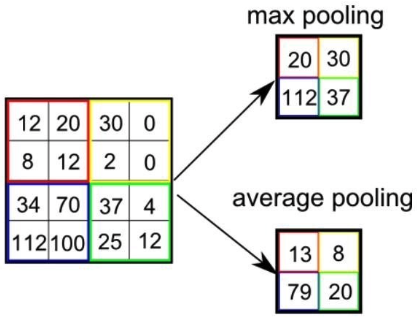
\includegraphics[width=5cm]{assets/pooling.png}
\end{center}

\subsection{Special Activation Functions}
Stacking many layers may lead to back-propagation problems, known as the \textbf{vanishing gradient problem}. For this reason, we use other activation functions.

\subsubsection{*LU Activation Functions}
In order to mitigate the back-propagation problem, we use special activation functions. Some of these are the \textbf{Rectified Linear Unit} (ReLU), the \textbf{Leaky Rectified Linear Unit} (Leaky ReLU), the \textbf{Scaled Exponential Linear Unit} (SELU), and the \textbf{Exponential Linear Unit} (ELU).

\subsubsection{Softmax Activation Function}
The softmax activation function takes a vector and turns it into the \textbf{membership probability} of the specific class. In other words, the network takes an image as input and outputs a vector representing a probability distribution over all the possible classes.
\[ \sigma (z)_j = \frac{e^{z_j}}{\sum^K_{k = 1}e^{z_k}} \]
Where $e^{z_j}$ is \textbf{one of the classes}.

\begin{center}
	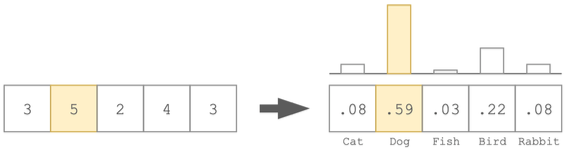
\includegraphics[width=8cm]{assets/softmax.png}
\end{center}
This is useful if used as the activation function of the last layer of a multi-class classifier.

\subsection{Loss Functions}
\subsubsection{Regression}
In the case of regression problems, the following are different loss functions:

\begin{itemize}
	\item \textbf{Mean Square Error (MSE)}
	\[ L(\theta) = \displaystyle\frac{1}{n} \sum^n_{i=1} (y_i - f(\theta,~x_i))^2 \]
	
	\item \textbf{Mean Absolute Error (MAE)}
	\[ L(\theta) = \displaystyle\frac{1}{n} \sum^n_{i=1} \left|y_i - f(\theta,~x_i)\right| \]
	
	\item \textbf{Mean Absolute Percentage Error (MAPE)}
	\[ L(\theta) = \displaystyle\frac{1}{n} \sum^n_{i=1} \frac{\left|y_i - f(\theta,~x_i)\right|}{y_i} \]
\end{itemize}

\subsubsection{Classification}
In the case of classification problems, we use the \textbf{cross-entropy} in order to compute the loss. The formula for the cross-entropy is the following:
\[ L(\theta) = \displaystyle -\frac{1}{n} \sum^n_{i=1}\sum^m_{j=1} y_{ij}\log(f(\theta,~x_i)_j) \]
The classification accuracy is the percentage of the correct predictions over the total predictions.

\subsection{Image Classification}
\subsubsection{AlexNet}
This was the first \textbf{deep convolutional neural network} to achieve good results on ImageNet. It is composed of several layers:

\begin{itemize}
	\item \textbf{Feature Extraction Layers}
	\begin{itemize}
		\item Convolutional Layer with a stride of 4
		\item Max Pooling Layers (x2)
		\item Fully Connected Layers (x2)
		\item Max Pooling Layer
	\end{itemize}
	
	\item \textbf{Application Specific Layers}
	\begin{itemize}
		\item Dense Layers with 4096 neurons (x2)
		\item Dense Layer with 1000 neurons
	\end{itemize}
\end{itemize}

\subsubsection{Very Deep Convolutional Neural Networks: VGG}
\textbf{Visual Geometry Group} (VGG) is a neural network that has been proposed in two variants: \textbf{VGG-19}, with 19 trainable layers, and \textbf{VGG-16}, with 16 trainable layers. \\ \\
\textbf{VGG-16} is still used today, as it provides a good tradeoff between accuracy, performance, and processing efficiency. The VGG-16 architecture is made up of several layers:

\begin{itemize}
	\item Convolutional Layers with a 3x3 receptive field mask and ReLU (x16)
	\item Max Pooling Layers (x5)
	\item Fully Connected Layers with ReLU (x3)
	\item Dense Layer with softmax
\end{itemize}
To \textbf{train} VGG-16, we use the \textbf{momentum term}. This means that if the previous update changes the weights by a significant margin, then the following update probably should remember that. Thus, the optimizer remembers the previous update and uses it to compute the new weights.
\[ \Delta\theta = \alpha\Delta\theta - \eta\displaystyle\frac{\partial V_n(\theta)}{\partial\theta}\Bigg|_{Z_n,i} \]
\[ \theta_{i+1} = \theta + \Delta\theta \]
In reality, a much more complex approach is used to optimize. This optimizer is called \textbf{Adam}. This algorithm does the following:

\begin{enumerate}
	\item Keeps a running average of the previous gradients and second moments
	\item Estimates the current gradient and the second moment using the running averages
	\item Updates the weights using the estimated values
\end{enumerate}
VGG can be trained using 32x32 batches, which is good enough and allows for better generalization.

\subsection{Autoencoders}
Encoders and decoders can comprise graph convolutional layers with pooling, dense feedforward neural networks, or other architectures. These encoders/decoders are used to learn a compact representation of the input space and filter out noise in the input data. \\ \\
After concept learning, autoencoders can generate novel patterns — known as generative schemes.

\begin{center}
	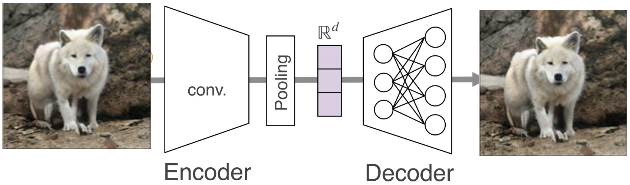
\includegraphics[width=9cm]{assets/encoders.png}
\end{center}

\section{Results from the Theory}
\subsection{Vapnik Chervonenkis Dimension}
If we consider a binary classification problem and a family of models $f(\theta, x)$, the Vapnik Chervonenkis (VC) dimension $d_{VC}$ is the \textbf{maximum} number of points for which there is a layout of points such that, for all points labelings, the classification provided by $f(\theta, x)$ makes no errors. \\ \\
In the classification case, if we consider the empirical risk as the ratio of correct classification on the training set, we have:
\[ Pr \left( \displaystyle \bar{V}(\hat \theta) \leq V_n(\hat \theta) + \sqrt{\frac{1}{n} \left[ d_{VC} \left( \log \left( \frac{2n}{d_{vc}} \right) + 1 \right) - \log \left( \frac{\delta}{4} \right) \right]} \right) \geq 1 - \delta \]
Which holds if $d_{VC} \ll n$

\subsection{Uniform Convergence of Empirical Mean}
The \textbf{empirical mean} converges to its expectation uniformly as $n$ goes to infinity, and for each element of an arbitrarily selected finite sequence of parameter estimates. \\ \\
From \textbf{Hoeffding inequality}, we have that:
\[ Pr \left( \sup_{L \in A} |V_n(L(\theta)) - E_x[L(\theta, x)]| > \varepsilon_V \right) \leq 2Me^{-2n\varepsilon^2_V} \]
\[ A = \{ L(\hat \theta_1, x), \dots, L(\hat\theta_M, x) \} \]
Provided that $M$ is finite, the right-most term goes to zero as $n$ tends to infinity. The \textbf{UCEM} property also holds for a family of functions composed of infinite models:
\[ A = \{ L(\theta, x), \theta \in \Theta \} \]
Provided the VC dimension is finite.

\subsection{The Bias-Variance Tradeoff}
We wish to evaluate the \textbf{expected test error} for a given $x$ and a quadratic loss function:
\[ SE_{PE}(x) = E[ y(x) - f(\hat\theta, x) ]^2 \]
The expectation is taken with respect to the realizations of the training set and the noise. The above formula can be rewritten as:
\[ SE_{PE} = \sigma^2_\eta + E \left[ (g(x) - E [f(\hat \theta, x)])^2 \right] + E \left[ (E[f(\hat \theta, x)] - f(\hat \theta, x))^2 \right] \]
The accuracy of the approximating model depends on three terms:

\begin{itemize}
	\item The \textbf{variance} of the noise
	\item The \textbf{bias}
	\item The \textbf{variance} associated with the training set
\end{itemize}
Some important notes about the above formula are:

\begin{itemize}
	\item The variance of the noise cannot be canceled out
	\item A model with high bias poorly approximates the unknown function
	\item A model family with high variance is susceptible to the particular selection of the training set
	\item As we use more flexible learning methods, the variance increases, and the bias decreases
\end{itemize}

\section{Other Classification Families}
\subsection{Classification and Regression Trees}
The input space is partitioned into regions, each associated with a constant value $\hat y_{R_i}$.

\subsubsection{Single-Component Splits}
The goal of CART is to learn the regions split. Since considering all possible region partitions is not feasible, we use heuristics based on incremental splits along single axes -- i.e., components. \\ \\
The regions are determined by a tree of splits, where two parameters define the splits:

\begin{itemize}
	\item $d$ -- The axis to split
	\item $t$ -- The threshold inducing the split
\end{itemize}

\begin{figure}[H]
   \begin{minipage}{0.48\textwidth}
     \centering
     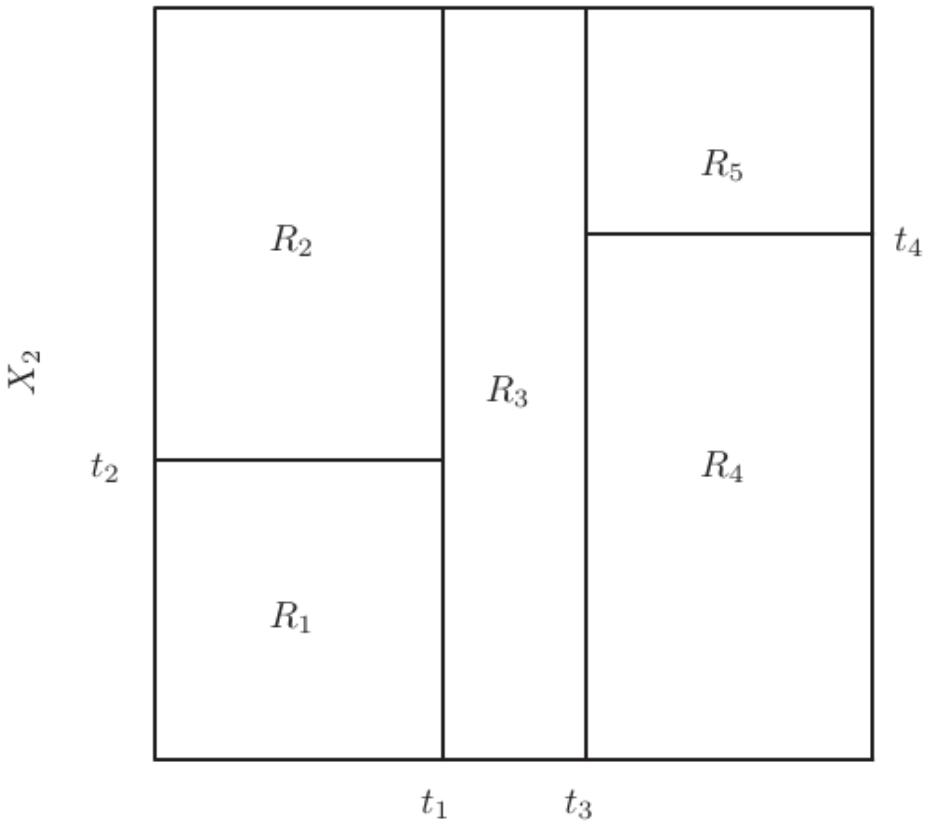
\includegraphics[width=.9\linewidth]{assets/cart.png}
   \end{minipage}\hfill
   \begin{minipage}{0.48\textwidth}
     \centering
     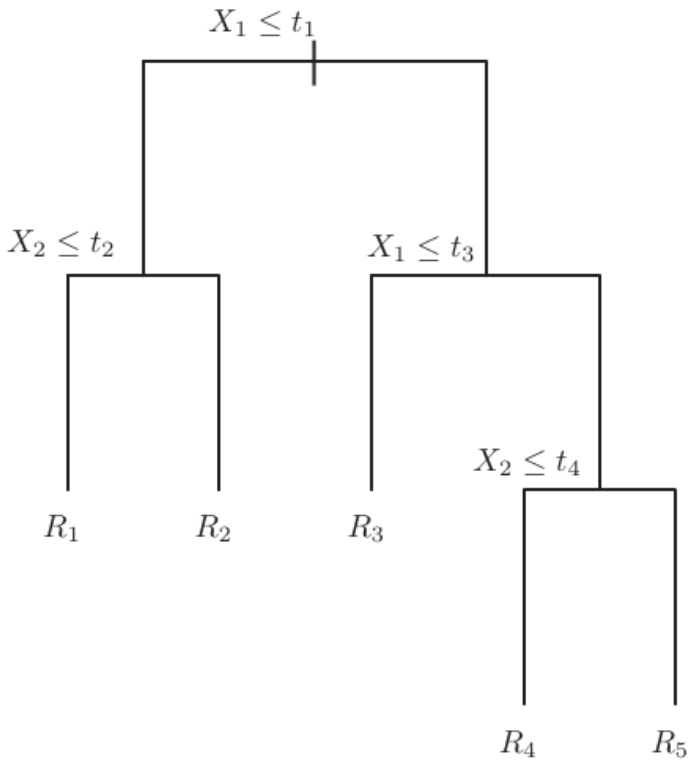
\includegraphics[width=.7\linewidth]{assets/cart_tree.png}
   \end{minipage}
\end{figure}

\subsubsection{Learning the Tree}
In CART, the region partitions are learned from the training set. \\ \\
To learn the tree, we use the \textbf{recursive binary splitting} heuristic. This process follows these steps:

\begin{itemize}
	\item Split along with a single component -- say $d$
	\item Each split results in two new tree branches. A region $R_{parent}$ is now split into two regions:
	\[ R_{left}(d, t) = R_{parent} \cap \{ x : x_d \leq t \} \]
	\[ R_{right}(d, t) = R_{parent} \cap \{ x : x_d > t \} \]
\end{itemize}
The thresholds $t$ are found by minimizing the estimated value $d$ and $t$. This can be done as such:
\[ \sum_{i \in R_{right}} L(y_i, \hat y_{R_{right}}; d, t) + \sum_{i \in R_{left}} L(y_i, \hat y_{R_{left}}; d, t) \]
This has to be repeated for all new regions and terminate with few data points -- although other termination criteria can be considered instead.

\subsubsection{Regression and Classification}
CART can be used in both regression and classification. For \textbf{regression}, the \textbf{prediction estimate} is the mean value:
\[ \hat y_{R_i} = \frac{1}{|R_i|} \sum _{j \in R_i} y_j \]
The \textbf{loss function} is the sum of squares:
\[ \displaystyle\sum_{i \in R_j}(y_i - \hat y_{R_j})^2 \]
For \textbf{classification}, the \textbf{prediction estimate} is the majority voting:
\[ \hat y_{R_i} = \displaystyle\arg\max_c\{ p_{R_i}(c) \} \]
Where $p_{R_i}(c)$ is the ratio of datapoints of class $c$ in region $R_i$. The \textbf{loss function} is the cross-entropy:
\[ - \sum_c p_{R_i}(c) \log(p_{R_i}(c)) \]

\subsection{Bagging}
Trees generate different models when trained on different datasets. By using bagging, we mitigate the high variance generated. When using this method, we do as follows -- in the case of regression:

\begin{itemize}
	\item We take $B$ independent training sets -- or use bootstrap.
	\item We build a model from each training set and generate a \textbf{forest}
	\item We consider the \textbf{ensemble} model
	\[ \hat f_{avg}(x) = \frac{1}{B}\sum^B_{b=1} \hat f^b(x) \]
\end{itemize}
This method is also known as \textbf{Random Forests}.

\subsection{Maximal Margin Classifier}
The criterion is not based on the data's density but the region of space occupied by the data -- i.e., their support. \\ \\
The dataset must be linearly separable for this method to be applied. To find a hyperplane that divides the data, we need to perform a maximization of margin $M$. This maximization is used to find the points near the margin. The vectors from these points and the hyperplane are known as \textbf{support vectors}.

\begin{center}
	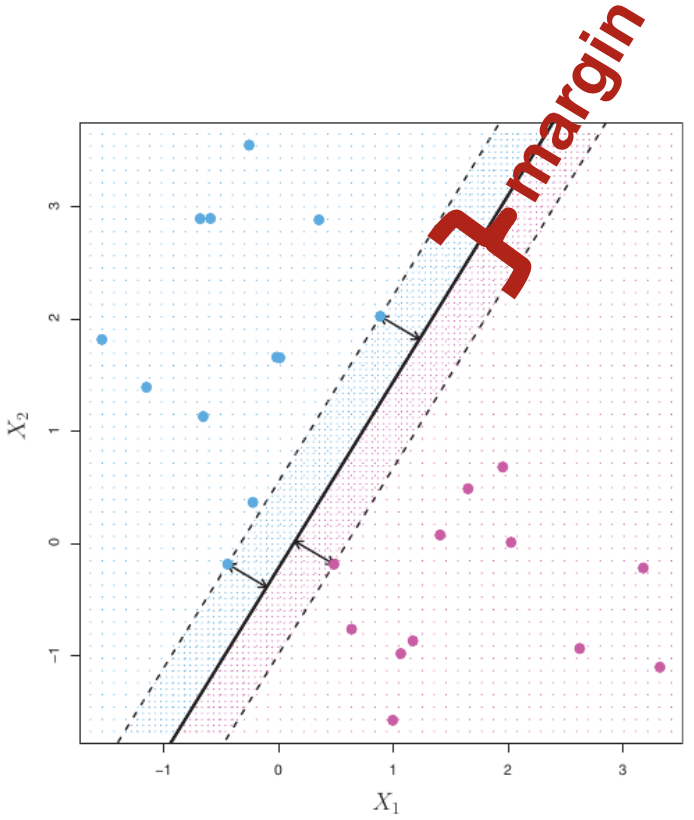
\includegraphics[width=4cm]{assets/mmc.png}
\end{center}

\subsection{Support Vector Classifier}
When data points are not linearly separable by a hyperplane, we introduce the \textbf{soft margin classifier} concept. \\ \\
With soft margins, we tolerate errors by introducing slack variables.
\[ \min_{w, \epsilon_i}||w||^2_2 + \lambda \displaystyle\sum^n_i \epsilon_i ~~~~~~~ \text{s.t.} ~ y_i(w^Tx_i + b) \geq 1 - \epsilon_i ~~~~~~~~ \text{with}~\epsilon_i \geq 0 \]
The hyperplane is determined only by those points on the wrong side of the plus-minus-hyperplane or those lying on them. Also in this case such vectors are known as \textbf{support vectors}.

\begin{center}
	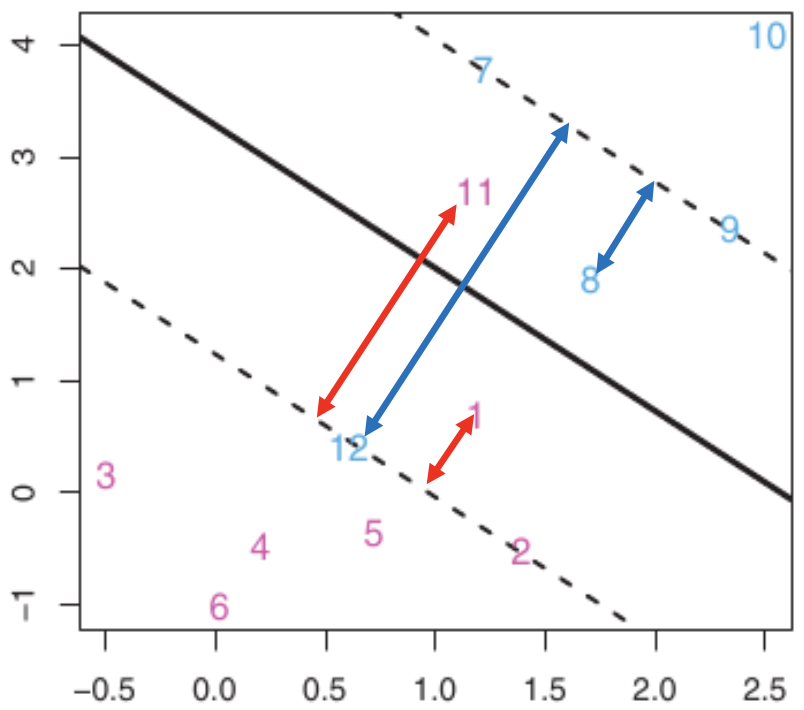
\includegraphics[width=5cm]{assets/svc.png}
\end{center}

\subsection{Support Vector Machines}
Some classification problems seem to be challenging to solve using linear methods. For this reason, we can \textbf{embed} the input data. This means that we can project the points onto a higher dimension. This will hopefully make the problem linearly separable, thus solvable.

\begin{center}
	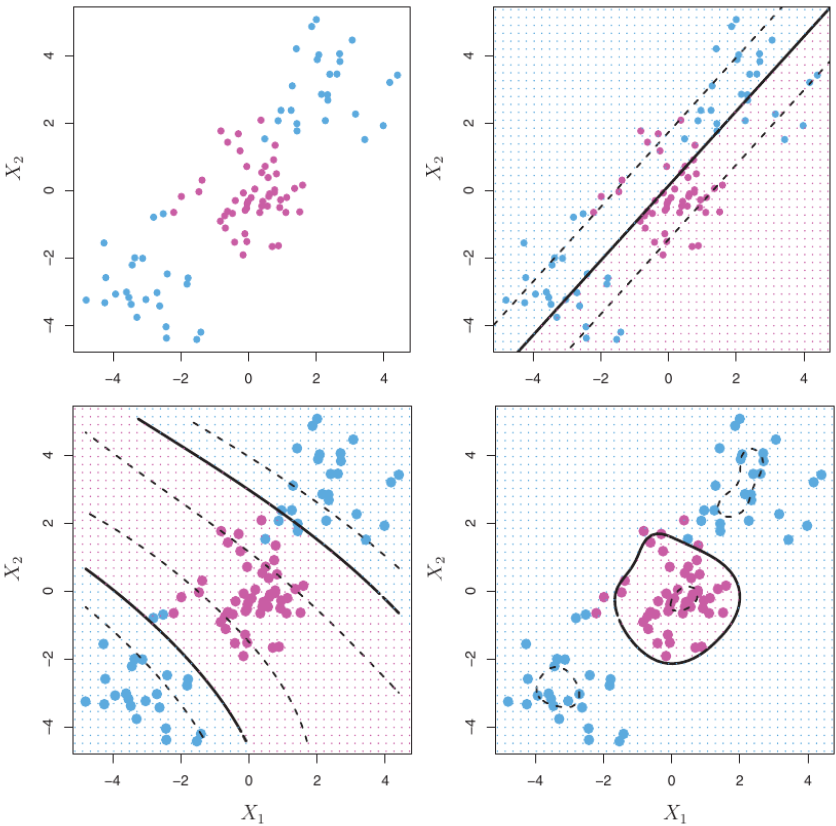
\includegraphics[width=8cm]{assets/svm.png}
\end{center}
The original soft-margin problem can be rewritten in the dual form:
\[ \max_{\alpha_i} \sum^n_{i=1} \alpha_i - \frac{1}{2} \sum^n_{i, j = 1} \alpha_i \alpha_j y_i y_j \langle x_i, x_j\rangle \]
\[ s.t. ~ 0 \leq \alpha_i \leq \lambda ~~~~~~~ \text{with} ~ \displaystyle \sum_i \alpha_i y_i = 0 \]
Which yields:
\[ \hat w = \displaystyle\sum^n_{i = 1} \alpha_i y_i x_i \]
By applying the embedding function $\phi(x)$ to $x$, the dual optimization problem now becomes:
\[ \displaystyle \max_{\alpha_i} \sum^n_{i=1} \alpha_i - \frac{1}{2} \sum^n_{i, j = 1} \alpha_i \alpha_j y_i y_j \langle \Phi(x_i), \Phi(x_j)\rangle \]
\[ s.t. ~ 0 \leq \alpha_i \leq \lambda ~~~~~~~ \text{with} ~ \displaystyle \sum_i \alpha_i y_i = 0 \]
The scalar product can now be substituted with a function named \textbf{kernel}. This function is the following:
\[ K(x_i, x_j) = \langle \Phi(x_i), \Phi(x_j) \rangle \]
Thus we can rewrite the dual optimization problem as:
\[ \displaystyle \max_{\alpha_i} \sum^n_{i=1} \alpha_i - \frac{1}{2} \sum^n_{i, j = 1} \alpha_i \alpha_j y_i y_j K(x_i, x_j) \]
\[ s.t. ~ 0 \leq \alpha_i \leq \lambda ~~~~~~~ \text{with} ~ \displaystyle \sum_i \alpha_i y_i = 0 \]
The classification can now be performed by checking the sign of the following:
\[ f(x) = \sum^n_{i = 1} \alpha_i y_i K(x, x_i) + \hat b \]
Where $\hat b$ is computed as:
\[ \hat b = y_* - \sum_i \alpha_i y_i K(x_i, x_*) \]

\subsubsection{Polynomial Kernel}
For the polynomial kernel, we consider the following polynomial of degree $d$:
\[ K(x, x') = (c + x^Tx')^d \]


\subsubsection{RBF Kernel}
For the Radial Basis Function kernel, we need to use the following function:
\[ K(x, x') = e^{-\gamma ||x-x'||^2} \]
Where the $\gamma$ value indicates the neighborhoods' tightness, this kernel's mapping space is infinitely dimensional.

\subsection{SVM VC Dimension}
In SVMs, the VC dimension $d_{VC}$ is upper-bounded by
\[ \frac{D}{M} \]
Where $D$ is the \textbf{diameter of the smallest sphere embracing the training points}, and $M$ is the \textbf{margin}.

\subsection{Multiclass Classification}
SVM only deals with binary classifiers. To tackle the multi-class problem, we need to train a classifier for each class. This means that the $n$-th classifier checks class $n$ against all the other classes. \\ \\
During the operational phase, we select the class for which the classification output is the farthest into the positive region.

\section{Unsupervised Learning}
In unsupervised learning, there no label/response $y$ is available. These algorithms need to discover the properties of a dataset given just a set of data points
\[ x_1, x_2, \dots, x_n \]

\subsection{Isolation Forest}
This is an interesting tree-based method designed to isolate anomalies explicitly. The assumption is that anomalies are rare events that differ from the nominal class ones. \\ \\
It is easier to isolate an anomalous point $x_0$ with respect to a genuine one $x_i$ when a $k$-dimensional tree is generated from data -- with a random splitting criterion. The anomalies will lie in \textbf{leaves with shallow depth}.

\begin{center}
	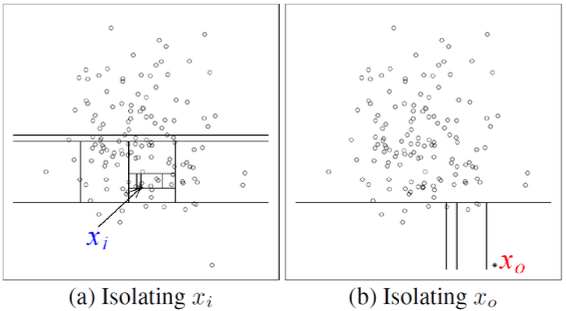
\includegraphics[width=6cm]{assets/ifor.png}
\end{center}

\subsubsection{Training}
To train an IFOR algorithm, we must first build a forest of trees given a dataset $X$. Now, for each of the training sets, we generate a tree as follows:

\begin{enumerate}
	\item Uniformly select an axis to split
	\item Determine a split point along the axis
	\item Stop the procedure when one of the following conditions are met:
	\begin{itemize}
		\item The tree reaches a depth limit
		\item The number  of points in the leaf equals 1
		\item The points in the leaves share the same values
	\end{itemize}
\end{enumerate}

\subsubsection{Operational Phase}
We compute the average path length:
\[ E(h(x)) \]
Among all the trees in the forest for the given point $x$. This point $x$ is identified as \textbf{anomalous}, if the anomaly score:
\[ s(x, n) = 2^{\frac{E(h(x))}{c(n)}} > T \]
Where $n$ is the number of \textbf{points in $X$}, $T$ is a \textbf{threshold}, and $c(n)$ is the \textbf{average path length} of generic binary trees given $n$ data instances
\[ c(n) = 2(\ln(n-1) + \gamma_E) - 2\frac{n-1}{n} \]
Where $\gamma_E$ is the \textbf{Euler-Mascheroni constant}. Moreover, the averaged path lengths of $x_i$ and $x_0$ \textbf{converge} when the number of trees in forest increase.

\subsection{Principal Component Analysis}
Principal Component Analysis changes the reference system of the data through a rotation operator. The axes of the new reference system show the most significant data scattering.

\begin{figure}[H]
   \begin{minipage}{0.48\textwidth}
     \centering
     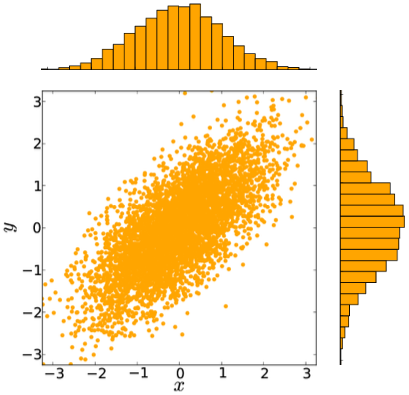
\includegraphics[width=.9\linewidth]{assets/pca.png}
   \end{minipage}\hfill
   \begin{minipage}{0.48\textwidth}
     \centering
     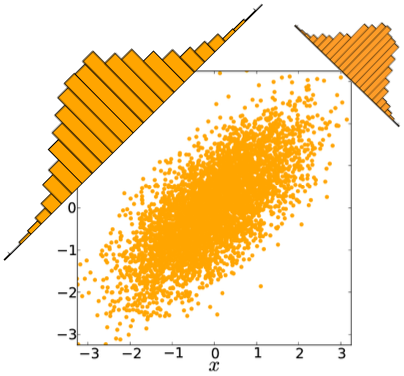
\includegraphics[width=.92\linewidth]{assets/pca1.png}
   \end{minipage}
\end{figure}
Given $d$-dimensional data points:
\[ x_1', x_2', \dots, x_n' \]
And centered data points:
\[ x_i = x_i' - \frac{1}{n} \sum_j x'_j \]
We will then have
\[ X = [x_1 | x_2 | \dots | x_n] \]
From this, we compute the sample covariance matrix and consider the symmetrical semidefinite positive matrix
\[ H = X^TX = U\Lambda U^T \]
Where $\Lambda$ is the matrix that contains all of the eigenvalues. Each eigenvalue corresponds to one dimension, and each component of
\[ \tilde x = U^Tx \]
It is called \textbf{principal component}.

\subsubsection{Dimensinality Reduction}
Once the data has been modified, we remove the smallest $l$ eigenvalues and group the remaining eigenvectors as:
\[ \tilde U = [ U_1 | U_2 | \dots | U_{l+1} ] \]
Dimensionality reduction is then obtained by means of:
\[ \tilde x = \tilde U^T x \]
As we embed the vectors from dimension $d$ into a lower $d-l$ dimension.

\subsubsection{Information Loss}
To determine how much information we lost from the PCA we use the \textbf{spectral decomposition}. The spectral decomposition theorem grants that:
\[ H = \sum^d_{i=1} \lambda_iU_iU_i^T \]
If we remove the smallest $l$ eigenvalues, we generate:
\[ \tilde H = \sum^d_{i = l+1} \lambda_iU_iU_i^T \]

\subsection{Clustering}
Sometimes the data group together in certain feature/input space regions. For this reason, we use \textbf{clustering}. Using this algorithm, we group data so that the points in the same cluster stay close.

\subsubsection{K-Means Clustering}
A \textbf{cluster} is defined as a set of indices such that
\[ C_k \subseteq \{ 1, 2, \dots, n \} \]
Given data points $x_1, x_2, \dots, x_n$, we perform the following steps:

\begin{enumerate}
	\item Randomly search for $K$ clusteroids $\mu_1, \mu_2, \dots, \mu_K$
	\item Given the selected clusteroids, create $K$ classes
	\item The points are then assigned to one of the clusters based on the Euclidean distance of the point to the clusteroids -- we need to find the minimum distance
	\item Recompute the clusteroids -- as the mean of the points in that cluster
	\item Perform steps 3 and 4 until the clusters converge -- there are no more changes in the clusters
\end{enumerate}


\end{document}

























